\chapter{Introdução}
\setcounter{page}{11}
A história de homens e animais domésticos é uma parceria antiga que acompanhou o desenvolvimento da civilização humana, proporcionando inúmeros benefícios. Mas aquilo que antes era apenas um vínculo de apoio ou segurança sofre grandes mudanças atualmente, principalmente devido ao controle de natalidade e ao processo de urbanização, fazendo com que os animais domésticos passem a assumir um papel diferenciado nas relações intrafamiliares, de modo que o proprietário chega a identificá-los como membros da família e proporcionam privilégios que antes eram partilhados apenas por seres humanos.
\\
\indent
De acordo com o crescimento populacional, muitos animais são adotados por um motivo sentimental, pois algumas pessoas acabam priorizando a atividade profissional, deixando para outro momento a formação de uma família.
\\
\indent
Os animais domésticos preenchem esse espaço, tornando assim uma transferência social mútua, na qual um complementa a vida um do outro, ou seja, há um beneficio para ambas as partes, como no mutualismo. Segundo os dados do Censo 2013 divulgados pelo IBGE (Instituto Brasileiro de Geografia e Estatística), aproximadamente 44,3\% (equivalente a 52,2 milhões) dos domicílios do país possuem pelo menos um cão e 17,7\% (equivalente a 11,5 milhões) possuem pelo menos um gato, fora outros animais criados nos lares brasileiros, que fazem com que esses números aumentem à cerca de 100 milhões. Isso confirma que há no Brasil mais animais domésticos do que crianças (45 milhões) até os onze anos. como dito por Juan Arias em uma coluna do jornal El País.
\\
\indent
Segundo o estudo liderado por Allen McConnel, da Universidade de Miami, publicado no site do Journal of Personality and Social Psychology, pessoas que convivem com animais de estimação "têm mais qualidade de vida e conseguem resolver melhor diferenças individuais que as que não têm animal de estimação" (Veja, 2011). O estudo também afirma que a criação de animais estimula o bom humor, a autoestima, a diversão,  afasta o sedentarismo e depressão, atuando ainda nos sentimentos de solidariedade, respeito, cumplicidade e amizade sejam adultas ou crianças melhorando em muito dos casos a qualidade de vida dos seus proprietários. Além disso, são demonstradas que grande parte das pessoas que convivem com animais vão menos ao médico e a recuperação de determinadas doenças tornam-se mais rápidas. 
\\
\indent
Mesmo com tantos benefícios, ainda há donos que não tratam seus animais com o devido cuidado, principalmente com relação a vacinas e medicamentos. Segundo os dados do censo do IBGE, cerca 75,4\% dos lares entrevistados nunca vacinaram seus animais ou deram a vacina num período de um ano antes da data de pesquisa. E isso ocorre muitas vezes por falta de informações necessárias que situem os donos, simplesmente por não haver uma integração comum, rápida e eficiente entre a comunidade de donos de animais de estimação, veterinários, clínicas e vendedores de produtos ou serviços, em conjunto com as mais variadas redes sociais.

\section{Problemática}

Um dos grandes problemas para quem tem animais de estimação é quando estes fogem, pois normalmente não possuem nenhuma identificação, causando uma experiência angustiante ao proprietário, a família e principalmente ao {\it pet} (animal), devido aos riscos que correm. Tornando ainda mais difícil quando se tem crianças em casa. Desesperados, muitos proprietários não sabem quais medidas tomar e pensam rapidamente em compartilhar fotos e dados do seu animal em redes sociais, sites de procura, entre outros. Mas, nem sempre há êxito em tais medidas.
\\
\indent
Outro dado importante, segundo a Associação pelos animais, é que desde 2005, a maioria desses {\it pets} perdidos são encontrados e recolhidos por pessoas comuns (Diferentes de veterinários, clínicas ou canis).


\begin{figure}[!htb]
	\centering
	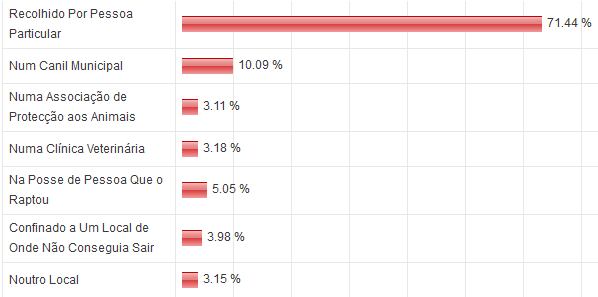
\includegraphics[scale=0.70
	]{imagens/animais}
	\caption{Animais Recolhidos}
	Fonte: encontra-me.org – Associação pelos animais. 2005 – 2015.
	\label{Rotulo}
\end{figure}
\newpage
Na maioria dos casos, as pessoas que encontram esses {\it pets} não imaginam que estes possuem proprietários, principalmente pelo animal não possuir nenhum mecanismo que os identifique. Assim essas pessoas acabam recolhendo os animais das ruas, para seus lares. 
\\
\indent
Além disso, o fato do animal não ter um sistema eficaz de identificação, dificulta bastante o seu tratamento, já que não é possível obter de forma eficaz aos seus históricos hospitalares, medicamentos, veterinários particulares e as clínicas mais confiáveis. Dificultando ainda o reconhecimento de doenças que o mesmo tem, impedindo assim, um tratamento ou a execução de uma cirurgia, caso este seja encontrado num difícil estado de saúde.  


\section{Objetivos Gerais}
\textbf{•} Desenvolver uma rede social diferenciada, capaz de integrar os animais de estimação ao meio social digital.
\\
\indent
\textbf{•} Proporcionar o aprendizado e a vivência de uma equipe de desenvolvimento com troca de experiências e conhecimento.

\section{Objetivos Específicos}
\textbf{•} Facilitar na identificação dos proprietários dos animais perdidos, para que esse seja comunicado acerca do seu pet, através do QR Code;
\\
\indent
\textbf{•} Proporcionar uma integração via rede social, que forneça uma maior praticidade numa consulta veterinária;
\\
\indent
\textbf{•} Exibir dados clínicos para que o veterinário fique ciente das medicações do animal e de doenças que ele teve em outras ocasiões;
\\
\indent
\textbf{•} Promover clínicas, veterinários, pet shops favoritos;
\\
\indent
\textbf{•} Permitir ao dono dos animais, compartilhar as tarefas diárias do seu animal, nas mais variadas redes sociais.

\section{Justificativas}

Como dito, observa-se que o mercado de animais de estimação é crescente, tornando-se necessária a promoção de ideias para esses novos serviços. Isso ocorre porque a cada dia é visível o aumento de benefícios que animais proporcionam aos humanos. Tornando assim, mais comum as famílias adotarem um {\it pet}, e tratá-los como verdadeiros membros da família.
\\
\indent
Sabe-se que os donos dos animais sempre procuram o melhor para os seus animais, mas muitas vezes acabam não conseguindo prover-lhes melhores condições. Nota-se também, que a sociedade atual está sempre rodeada por tecnologia, seja utilizando redes sociais, aplicativos móveis dentre outros.
\\
\indent
Portanto, identificando a importância desses pontos para a sociedade atual, o ePuppy surge como uma rede social buscando, conciliar as mais variadas comunidades (clínicas, veterinários e vendedores de produtos e serviços) com os proprietários que buscam sempre o melhor para os seus {\it pets}, seja no aprofundamento de informações, consultas e serviços diferenciados (gerenciador de e-mails e compartilhamento de conhecimento), facilitando também o encontro destes, por meio de coleiras personalizadas com {\it QR Code}.

\section{Metodologia}
Esta seção descreverá toda a metodologia utilizada para o desenvolvimento do ePuppy.

\subsection{PHP}
O ePuppy foi desenvolvido na linguagem de programação PHP (um acrônimo recursivo para {\it PHP: Hypertext Preprocessor}, originalmente Personal Home Page), disponível no site (www.php.net), na versão 5.5.9. 

\begin{figure}[!htb]
	\centering
	
\includegraphics[scale=0.50
	]{imagens/php_logo}
	\caption{Logo PHP}
	Fonte: Site Oficial do PHP.
	\label{Rotulo}
\end{figure}

Criada em 1995 por Rasmus Lerdorf, é uma linguagem interpretada usada para criação de aplicações que executam no lado do servidor, capazes de gerar conteúdo dinâmico em páginas que utilizam linguagem de marcação HTML (em acrônimo para {\it HyperText Markup Language}). A vantagem é que páginas HTML (Freeman e Freeman, 2006) podem ser interpretadas por navegadores {\it web} tradicionais, como por exemplo: Firefox, Chrome, Internet Explorer, Safari ou Opera.


\subsection{CakePHP}
O esforço de desenvolvimento do projeto foi minimizado com a utilização do {\it framework} CakePHP, disponível no site (www.cakephp.org), na versão 2.5.5. 

\begin{figure}[!htb]
	\centering
	
\includegraphics[scale=0.50
	]{imagens/cake-logo}
	\caption{Logo CakePHP}
	Fonte: Site Oficial do CakePHP.
	\label{Rotulo}
\end{figure}

Um {\it framework}, em linhas gerais, é uma abstração que une códigos comuns entre vários projetos de software provendo uma funcionalidade genérica, que pode atingir uma funcionalidade mais específica, por configuração, durante a programação de uma aplicação. O CakePHP foi desenvolvido em 2009 por Garrett Woodworth. É escrito na linguagem de programação PHP e tem como principais objetivos oferecer uma estrutura que possibilite aos programadores de todos os níveis, contemplando os alunos iniciantes do instituto federal, desenvolverem aplicações robustas rapidamente, mas sem perder flexibilidade.
\\
\indent
A escolha foi motivada pelo fato do CakePHP utilizar conceitos de Engenharia de Software e Padrões de Projetos bem-conhecidos (Fowler, 2003; Gamma, 1994), tais como: {\it Active Record, Association Table Mapping, Front Controller e Model-View-Controller (MVC)}.

\subsection{MySQL}
Os dados dos usuários (Proprietários, clinicas e veterinários), animais, plublicações, históricos de consultas, e-mails entre outras, funcionam on-line e os esses são guardados de forma segura no banco de dados MySQL, disponível no site (www.mysql.com), na versão 5.5.43. 

\begin{figure}[!htb]
	\centering
	
\includegraphics[scale=0.50
	]{imagens/logo-mysql}
	\caption{Logo MySQL}
	Fonte: Site Oficial do MySQL.
	\label{Rotulo}
\end{figure}

O MySQL foi desenvolvido em 1995 por David Axmark, Allan Larsson e Michael Monty, e utiliza a linguagem de consulta SQL (um acrônimo para {\it Structured Query Language}) como interface. Vários motivos nos levaram a escolha desse banco de dados, dentre eles: integração nativa com a linguagem PHP, excelente desempenho, estabilidade e suporte para qualquer plataforma atual (Suehring, 2002).


\subsection{Git e BitBucket}
Para o controle de versionamento do sistema, utilizamos o Git, disponível no site (www.git-scm.com), na versão 2.6.2. 

\begin{figure}[!htb]
	\centering
	
\includegraphics[scale=0.10
	]{imagens/logo_git}
	\caption{Logo Git}
	Fonte: Site Oficial do Git.
	\label{Rotulo}
\end{figure}

Um sistema de controle de versão com a possibilidade de gravar documentações e comentários. O Git foi desenvolvido inicialmente por Linus Torvalds em 2005 com a finalidade de versionalizar projetos visando uma maior, velocidade, {\it design} simples, com Suporte robusto a desenvolvimento não linear (milhares de {\it branches} paralelos), distribuído e capaz de lidar eficientemente com grandes projetos como o {\it kernel} do Linux (velocidade e volume de dados).
\\
\indent 
Em conjunto com o Git, utilizamos o BitBucket em sua versão gratuita, encontrado no {\it link} (www.bitbucket.org).

\begin{figure}[!htb]
	\centering
	
\includegraphics[scale=0.50
	]{imagens/bitbucket-logo}
	\caption{Logo BitBucket}
	Fonte: Site Oficial do BitBucket.
	\label{Rotulo}
\end{figure}

 É um site que visa hospedar projetos, utilizando o Git como o controlador de versão. O BitBucket foi desenvolvido em 2008 com Python. A escolha foi motivada pelo fato do BitBucket disponibilizar uma versão gratuita com espaço ilimitado e com capacidade para 5 programadores, caso o projeto seja privado, se não, o bitbucket também disponibiliza quantidade ilimitada de programadores.


\subsection{Editores de Texto Utilizados}	
	Toda a codificação do projeto foi desenvolvida com a utilização dos editores, Atom (versão 1.0) e Brackets (1.0).
\\
\indent
O Atom é um editor de código fonte livre e de código aberto para OS X, Linux e Windows e foi desenvolvido em 2014 pela GitHub. A escolha pelo editor foi incentivada pelo fato de suporte para plugins escritos em Node.js e principalmente pela incorporação de controle Git, mostrando os arquivos modificados de acordo com o Git.
\begin{figure}[!htb]
	\centering
	
\includegraphics[scale=0.05
	]{imagens/atom_logo}
	\caption{Logo Atom}
	Fonte: Site Oficial do Atom.
	\label{Rotulo}
\end{figure}
\\
\indent
O Brackets é um editor de texto open source e moderno, para criação e edição de arquivos (IDE) HTML, CSS, JS e PHP. Foi desenvolvido pela Adobe e tem como principais atributos, atualizações em tempo real (quando em conjunto com o Chrome), instalador de extensão e possibilidade de personalização de recursos.
\begin{figure}[!htb]
	\centering
	
\includegraphics[scale=0.05
	]{imagens/brackets_logo}
	\caption{Logo Brackets}
	Fonte: Site Oficial do Brackets.
	\label{Rotulo}
\end{figure}

\subsection{Ambiente de Trabalho}
Uma vez escolhidas as tecnologias a serem utilizadas, foi então organizado o ambiente de desenvolvimento. O projeto foi desenvolvido em 3 computadores pessoais ({\it notebook}) e 3 computadores de mesa ({\it desktop}), no laboratório de pesquisa de informática do campus Natal – Zona Norte. Os {\it notebooks} tinham processadores Intel Core i5, 4 GB de memória RAM, executando o sistema operacional Linux, distribuição Ubuntu, Voyager ou Arch Linux. Os computadores pessoais tinham processadores AMD Athlon, 4 GB de memória RAM, executando o sistema operacional Windows 7.	

\subsection{Processo de Contrução}
O processo de construção do sistema ePuppy foi realizado sempre com a divisão de grupos, denominados {\it Back-End} (responsáveis pela codificação e interligação dos códigos com a interface) e {\it Front-End} (Responsáveis pela criação da interface). A codificação do sistema foi totalmente distribuída em pares, na qual, duas pessoas codificam as mesmas coisas, amenizando os erros que podem ocorrer durante o processo devido a permanente inspeção de código que ocorre durante seu uso.
\\
\indent
Além dessa divisão, segmentou-se a construção do ePuppy em cinco etapas (Sommerville, 2011): (I) levantamento de requisitos, (II) modelagem, (III) codificação, (IV) teste e (V) implantação. Porém, o andamento do projeto está entre as etapas (III) e (IV), ou seja, as etapas de codificação e testes dos códigos que estão sendo projetados.
\\
\indent
	A etapa (I), foi dedicada ao entendimento das necessidades de um cliente em potencial, bem como, foi estudada a viabilidade de desenvolvimento do projeto. Foram realizados entrevistas e a formulação de questionários com dois profissionais da área e com proprietários de animais, para que pudéssemos realizar o levantamento dos requisitos necessários para a formação da ideia. Uma vez alcançado um entendimento geral do projeto, foram conduzidas reuniões com os mesmos profissionais para validar as especificações levantadas, e então definir uma especificação final isenta de ambiguidades, para a produção do relatório final da etapa (Documento de Requisitos). Os questionários e documento final foram elaborados utilizando apenas o editor de texto LibreOffice Writer, disponível no site (www.libreoffice.org), na versão 4.2.8.2.
\\
\indent
Já na etapa (II), uma vez que foram definidos os requisitos funcionais e não-funcionais do sistema, foi dado início à modelagem. Em outras palavras, foram produzidos os diagramas de caso de uso e de classe (Fowler, 2005; Bezerra, 2002). O primeiro diagrama permite literalmente, desenhar o processo de execução do negócio e visualizar a responsabilidade de cada participante (atores), quando ele entrará em cena, qual a sua interação, a amplitude e a sequência em que seu trabalho precisa ser realizado em relação às responsabilidades e tarefas dos demais integrantes do processo. O segundo diagrama faz uma representação da estrutura e relações das classes que servem de modelos para os objetos. Para a construção dos diagramas, foi utilizado o editor Astah, disponível no site (www.astah.net), na versão 7.0.0.
\\
\indent
Na etapa (III), foi realizada a escrita efetiva do programa. Foi utilizado os editores de textos Atom e Brackets para codificação, disponíveis nos sites (www.atom.io) e (www.brackets.io), nas versões 1.0. Cada versão do programa foi controlada e gerenciada com o uso do programa Git, disponível no site (www.git-scm.com), na versão 2.6.2. Para permitir o desenvolvimento colaborativo entre os programadores, o projeto utilizou o serviço de {\it web hosting} do Bitbucket (https://usuário@bitbucket.org/epuppyteam/epuppy.git).
\\
\indent
A etapa (IV) foi dedicada a vasculhar todo o projeto na tentativa de encontrar possíveis falhas de codificação. A fim de fornecer informações sobre a qualidade do produto em relação ao contexto em que ele deve operar. Os aspectos de qualidade inicialmente investigados são: funcionalidade e usabilidade. Nos testes de funcionalidade, são criados testes automáticos de unidade com PHPUnit, disponível no site (www.phpunit.de), na versão 4.7, na tentativa de se verificar as menores unidades de software (sub-rotinas, métodos, classes ou pequenos trechos de código). O objetivo do teste é encontrar falhas de funcionamento dentro de uma pequena parte do sistema funcionando independente do todo. Já em relação à usabilidade, analisamos a capacidade do produto ser facilmente compreendido, seu funcionamento aprendido, ser operado e atraente ao usuário. Os testes de usabilidade são realizados com usuários em potencial do sistema, a partir de protótipos ou na própria aplicação sendo executada no ambiente de desenvolvimento.
\\
\indent
Por fim, a etapa (V) disponibilizará o sistema ePuppy em produção para ser utilizado efetivamente. Para essa etapa, será primeiramente realizado o registro do domínio. Em seguida, o sistema será hospedado, num serviço que suporte as tecnologias PHP e MySQL, facilitando o gerenciamento do sistema de forma {\it on-line}. Assim o ePuppy estará pronto para ser acessado pelos demais usuários.


\section{Organização do Documento}

O presente trabalho está moldado em seis capítulos. Através desde capítulo, foi apresentada a introdução do trabalho, relacionando justificativa, problemática, objetivos e metodologia utilizada. No segundo capítulo (Fundamentação Teórica), será apresentado o embasamento do trabalho de acordo com alguns estudiosos da área. Ao longo do capítulo 3 (Redes sociais e o ePuppy), será abordado uma breve pesquisa sobre redes sociais, e suas principais características, relacionando com o ePuppy e sistemas relacionados. O capítulo 4 (Análise dos requisitos), discorrerá sobre as principais formas de elicitação de requisitos utilizadas, casos de uso e diagramas e entidade-relacionamento. O capitulo 5 (Análise dos resultados), descreverá toda a funcionalidade implementadas no sistema. E o capítulo 6 (Considerações Finais), apresentará as conclusões embasadas nas pesquisas realizadas e sugestões para trabalhos futuros.
